\begin{pregunta}
\begin{cuerpo}
Conidere los siguientes valores
$$
x_0=-2,\qquad x_1=0,\qquad x_2=1,\qquad x_3=3,
$$
y $l_0, l_1, l_2, l_3$ los respectivos \textbf{polinomios de Lagrange} asociados a estos valores. Considere tambi\'en la gr\'afica:
\medskip

\centerline{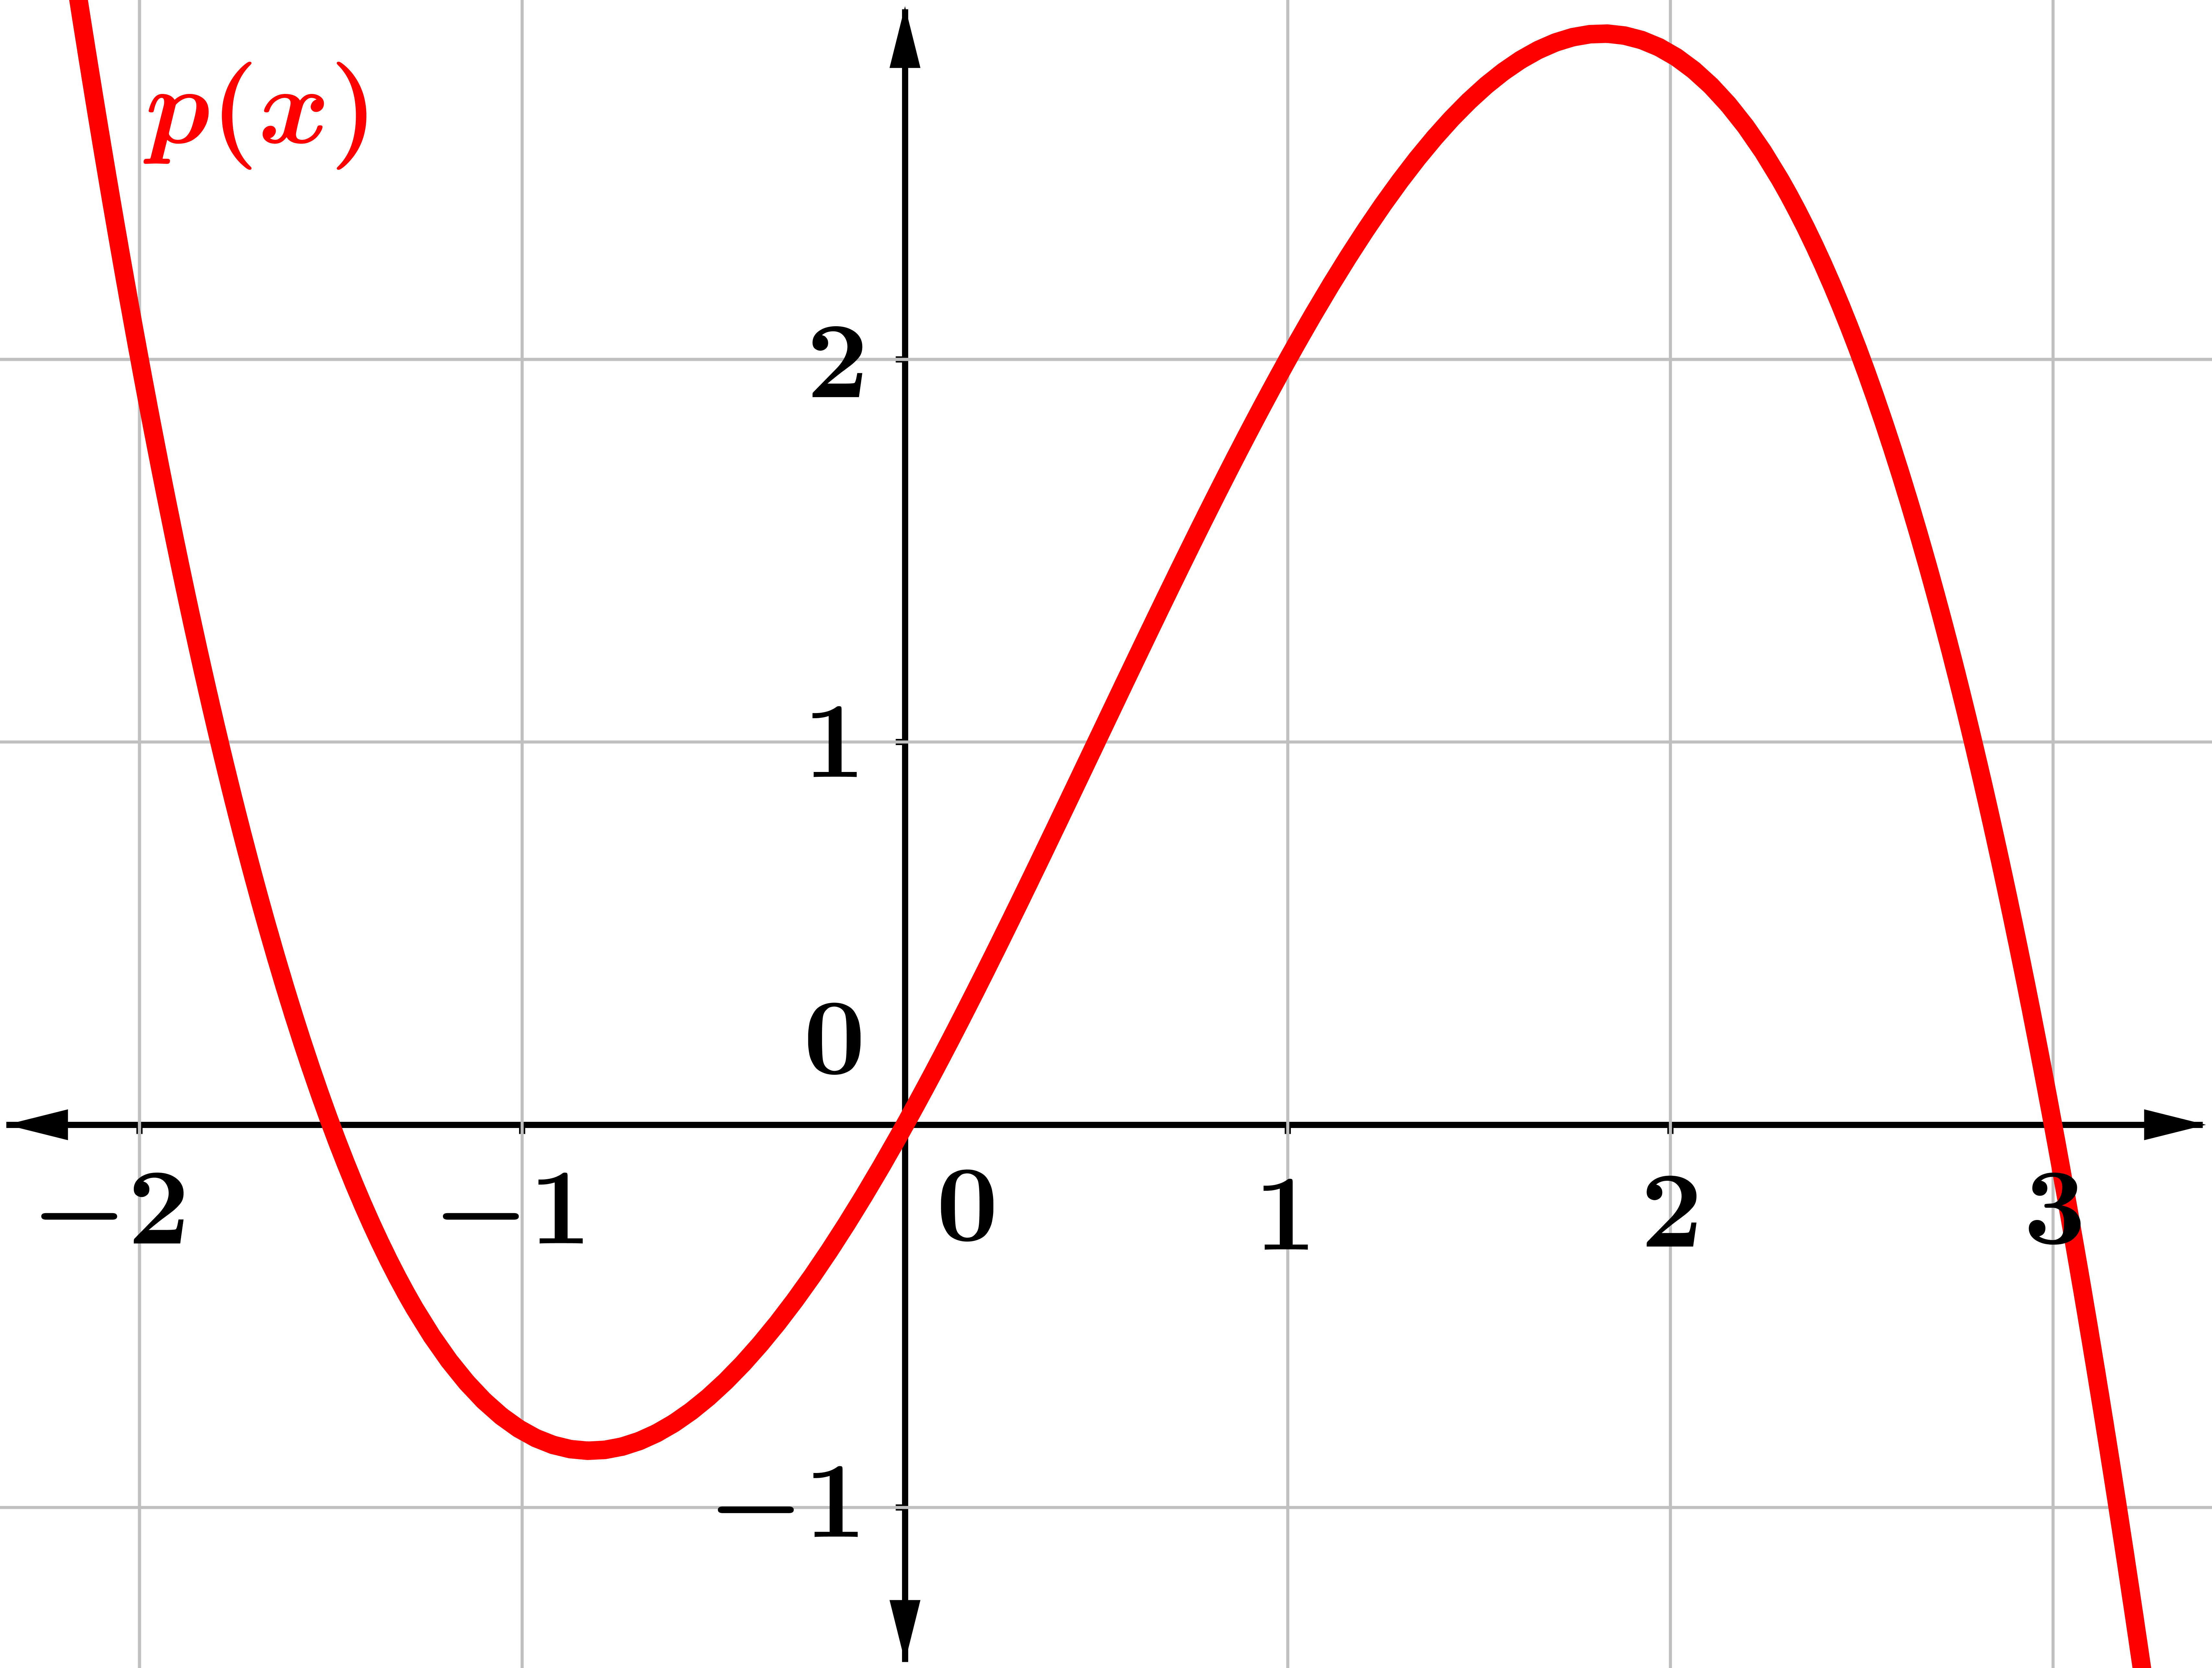
\includegraphics[width=0.4\textwidth]{./img/lagrange.png}}
\medskip

>A cu\'al de las siguientes funciones corresponde la gr\'afica anterior?
\end{cuerpo}
\begin{multicols}{2}
\begin{alternativas}
{$p(x)=2l_0(x)+2l_2(x)$}
{$p(x)=2l_1(x)+2l_3(x)$}
{$p(x)=2l_0(x)+2l_3(x)$}
{$p(x)=2l_1(x)+2l_2(x)$}
\end{alternativas}
\end{multicols}
\justificacion{0cm}
\end{pregunta}